\documentclass[10pt,xcolor=pdflatex,hyperref={unicode}]{beamer}
\usepackage{newcent}
\usepackage[utf8]{inputenc}
\usepackage[slovak]{babel}
\usepackage[T1]{fontenc}
\usepackage{pict2e}
\usepackage{amsthm}
\usepackage{graphicx}
\usepackage{amsmath}
\usepackage{hyperref}
\usepackage{fancyvrb}

\usepackage[ruled,czech,noline,longend,linesnumbered]{algorithm2e}

\usetheme{Warsaw}
\usecolortheme{beaver}
\setbeamertemplate{navigation symbols}{} 
\setbeamertemplate{footline}[frame number]

\title{Merge sort}
\subtitle{Typografie a publikování \,--\, 5. projekt}
\author{Peter Ďurica}
\institute{Vysoké učení technické v~Brně\\Fakulta informačních technologií}
\date{\today}

\begin{document}

\frame[plain]{\titlepage}

\begin{frame}
\frametitle{Výhody Merge sort}
Výhody Merge sort oproti ostatným algoritmom:\pause
\begin{itemize}
 \item<2->Je rýchlejší pre väčšie zoznamy, pretože narozdiel od insertion a bubble sortu neprechádza cez zoznam viac krát.
 \item<3-> Je stabilný, teda 2 elementy zoznamu s~rovnakou hodnotou si zachovajú svoje poradie vo finálnom zozname.
 \item<4-> Má konštantnú zložitosť.
\end{itemize}
\pause\pause\pause
Nevýhody Merge sort:
\begin{itemize}
 \item<6-> Pomalší pre menšie zoznamy, kvôli konštantnej zložitosti.
 \item<7-> Používa viac pamäte kvôli tvorbe finálneho zoznamu. Nepracuje \alert{in situ}.
\end{itemize}
\end{frame}

\begin{frame}
\frametitle{Princíp Merge sort}
Merge sort je založený na princípe \alert{zlučovania}.
\begin{itemize}
    \item Pole rozdeľujeme do tzv. \alert{behov} – súvislých úsekov, ktoré sú už zoradené.
    \item Na začiatku budú všetky behy jednoprvkové.
    \item Potom budeme dohromady zlievať vždy dva susedné behy do jediného zoradeného behu o~dĺžke danej súčtom počtu prvkov zlievaných behov, ktoré bude ležať na mieste oboch vstupných behov.
    \item V~poslednej iterácii bude postupnosť pozostávať z~jediného behu, a bude teda \alert{zoradená}.
\end{itemize}
Rekurzívna varianta – metóda postupne volá samú seba pre ľavú a
pravú polovicu zadanej časti pola a pri návrate z~rekurzie zlieva už
roztriedené postupnosti.
\end{frame}

\begin{frame}
\frametitle{Vizualizácia Merge sort}
\begin{block}{Postup}
Merge sort najskôr rozdelí zoznam na jednoprvkové hodnoty, ktoré následne zoradí do postupne väčších postupností až sa dopracuje k~jednému finálnemu zoznamu.
\end{block}
\begin{center}
    \scalebox{0.35}{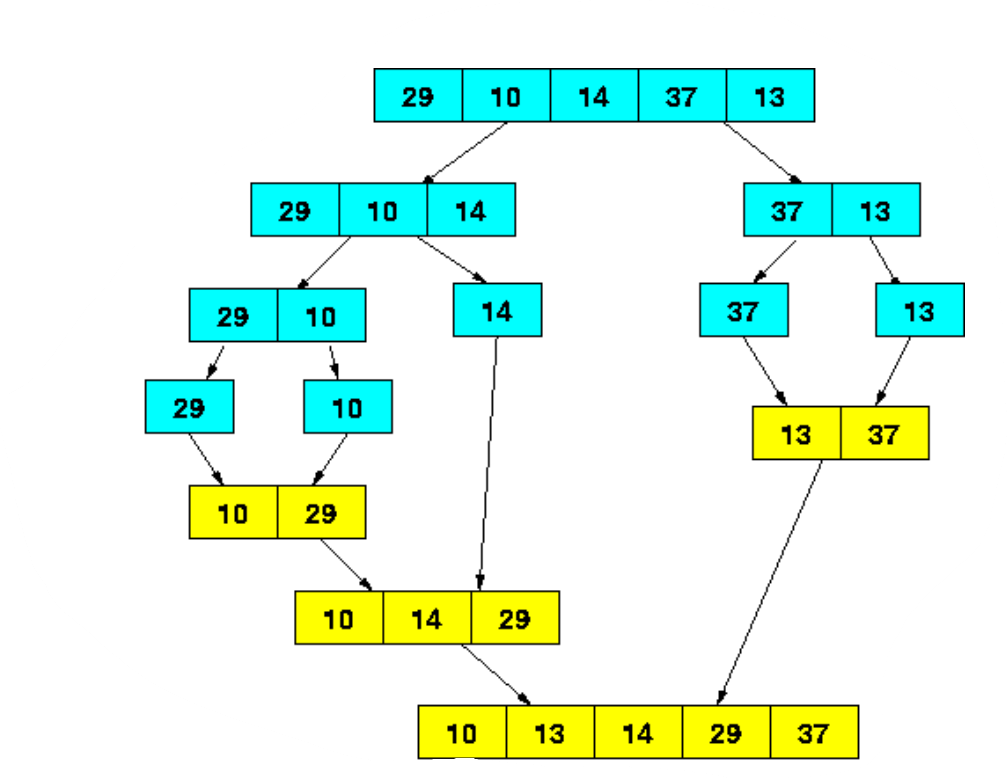
\includegraphics{visual.png}}
\end{center}
\end{frame}

\begin{frame}
\frametitle{Pseudokód Merge sort}
\begin{algorithm}[H]
\NoCaptionOfAlgo
\DontPrintSemicolon
	\If{$n == 1$}{
	    return a
	}\;
	\textbf{var} l1 \textbf{as} array = $a[0]$ \dots $a[n/2]$\;
	\textbf{var} l2 \textbf{as} array = $a[n/2+1]$ \dots $a[n]$\;
	\;
	l1 = mergesort( l1 )\;
	l2 = mergesort( l2 )\;
	\;
	\textbf{return} merge( l1,l2 )\;
	\caption{\textbf{function} mergesort(\textbf{var} a \textbf{as} array)}
\end{algorithm}
\end{frame}

\begin{frame}
\frametitle{Pseudokód Merge sort}
\begin{algorithm}[H]
\NoCaptionOfAlgo
\DontPrintSemicolon
    \textbf{var} c \textbf{as} array\;
    \While{a \textbf{and} b have elements}{
        \uIf{$a[0] > b[0]$}{
            \textbf{add} $b[0]$ to the \textbf{end of} c\;
            \textbf{remove} $b[0]$ \textbf{from} b\;
        }
        \Else{
            \textbf{add} $a[0]$ to the \textbf{end of} c\;
            \textbf{remove} $a[0]$ \textbf{from} a\;
        }
    }
	\caption{\textbf{function} merge(\textbf{var} a \textbf{as} array, \textbf{var} b \textbf{as} array)}
\end{algorithm}
\end{frame}

\begin{frame}
\frametitle{Pseudokód Merge sort}
\begin{algorithm}[H]
\NoCaptionOfAlgo
\DontPrintSemicolon
\setcounter{AlgoLine}{10}
    \While{a has elements}{
        \textbf{add} $a[0]$ to the \textbf{end of} c\;
        \textbf{remove} $a[0]$ \textbf{from} a\;
    }
    \;
    \While{b has elements}{
        \textbf{add} $b[0]$ to the \textbf{end of} c\;
        \textbf{remove} $b[0]$ \textbf{from} b\;
    }
    \;
    \textbf{return} c\;
    \caption{Pokračovanie \textbf{function} merge}
\end{algorithm}
\end{frame}

\begin{frame}
\frametitle{Zložitosť Merge sort}
    Merge sort má zložitosť \alert{O(n*log~n)}.
    \begin{itemize}
        \item Ak každým krokom delíme číslo na polovice, tak sa to označuje logaritmickou funkciou \alert{log~n} a počet krokov sa reprezentuje najviac \alert{log~n~+~1}.
        \item Takisto spravíme jednokrokovú operáciu pri hladaní stredu zoznamu. tj. \alert{O(1)}
        \item Pre spojenie predtým rozdelených zoznamov potrebujeme zložitosť \alert{O(n)}.
        \item Takže celkový čas za ktorý sa vykoná Merge sort bude \alert{n(log~n~+~1)}, čo nám dá zložitosť \alert{O(n*log~n)}.
    \end{itemize}
    Keďže Merge sort má konsťantnú zložitosť tak to znamená že v~najhoršom aj v~najlepšom prípade sa jej hodnota nemení.
\end{frame}

\begin{frame}
\frametitle{Porovnanie zložitostí algoritmov}
Porovnanie zložitosti Merge sortu s~ostatnými riadiacimy algoritmami:
\begin{center}
    \scalebox{0.4}{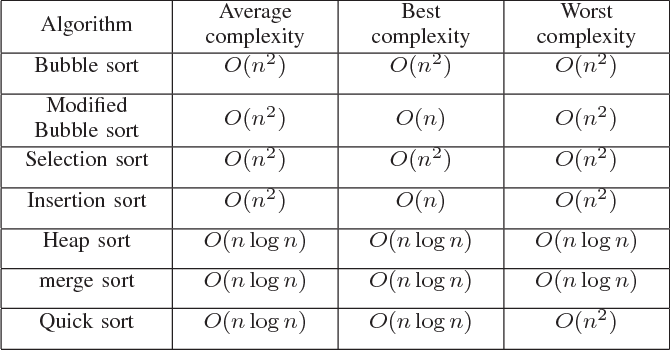
\includegraphics{complexities.png}}
\end{center}
\end{frame}

\begin{frame}
\frametitle{Použité zdroje}
\begin{itemize}
    \item Data Structures - Merge Sort Algorithm \\
    \href{https://www.tutorialspoint.com/data_structures_algorithms/merge_sort_algorithm.htm}{\scriptsize\texttt{https://www.tutorialspoint.com/merge-sort-algorithm.htm}}
    \item Merge sort, advantages and disadvantages \\
    \href{https://getrevising.co.uk/grids/merge-sort-advantages-and-disadvantages}{\scriptsize\texttt{https://getrevising.co.uk/merge-sort-advantages-and-disadvantages}}
    \item Quick Sort vs Merge Sort\\
    \href{https://www.geeksforgeeks.org/quick-sort-vs-merge-sort/}{\scriptsize\texttt{https://www.geeksforgeeks.org/quick-sort-vs-merge-sort/}}
    \item Prezentácia z~8.prednášky predmetu IAL
    \item Obrázok zložitosti algoritmov
    \href{https://www.semanticscholar.org/paper/An-efficient-hardware-implementation-of-odd-even-Korat-Yadav/6538996857d08bc96d73ef6f3db1f3f54599a074/figure/5}{\scriptsize\texttt{https://www.semanticscholar.org/paper/}}
\end{itemize}
\end{frame}
\end{document}
